Algoritmos como K-Means presentan dificultades para identificar clusters cuando las distancias entre elementos de un mismo conjunto es mayor que la de elementos de conjuntos distintos.
En estos casos, puesto que K-Means busca minimizar la distancia entre los elementos dentro de un mismo cluster, producirá clusters que difieran significativamente de los grupos <<correctos>>.
Tal es el caso de conjuntos cuyos elementos se encuentran distribuidos siguiendo formas que difieren significativamente de las de una esfera en el hiperplano correspondiente, como podemos apreciar en la figura. %TODO Add figure

En la imagen podemos observar asimismo el comportamiento de otro algoritmo sobre el mismo conjunto de datos.
En esta sección abordamos el algoritmo en cuestión, denominado \textit{DBSCAN}~\footnote{Siglas en inglés de \textit{Density-based spatial clustering of applications with noise}.}, que forma parte del conjunto de algoritmos de clustering basados en la densidad de los datos.

Un cluster basado en el criterio de densidad de los puntos consiste en un área densa de puntos conectados, separado de otros clusters por áreas de menor densidad.

\subsection{Densidad}\label{subsec:densidad}

El algoritmo DBSCAN define la densidad alrededor de un punto como la cantidad de puntos localizados alrededor de este en un radio, $Eps$, específico.
El propio punto es incluido en este conteo.
En la figura~\ref{img:dbscan} se puede observar gráficamente esta definición.
En este caso número de puntos alrededor de $A$ es 7.

El valor del radio es determinante en la densidad de un punto; si este valor es suficientemente grande

\begin{figure}[!h]
    \centering
    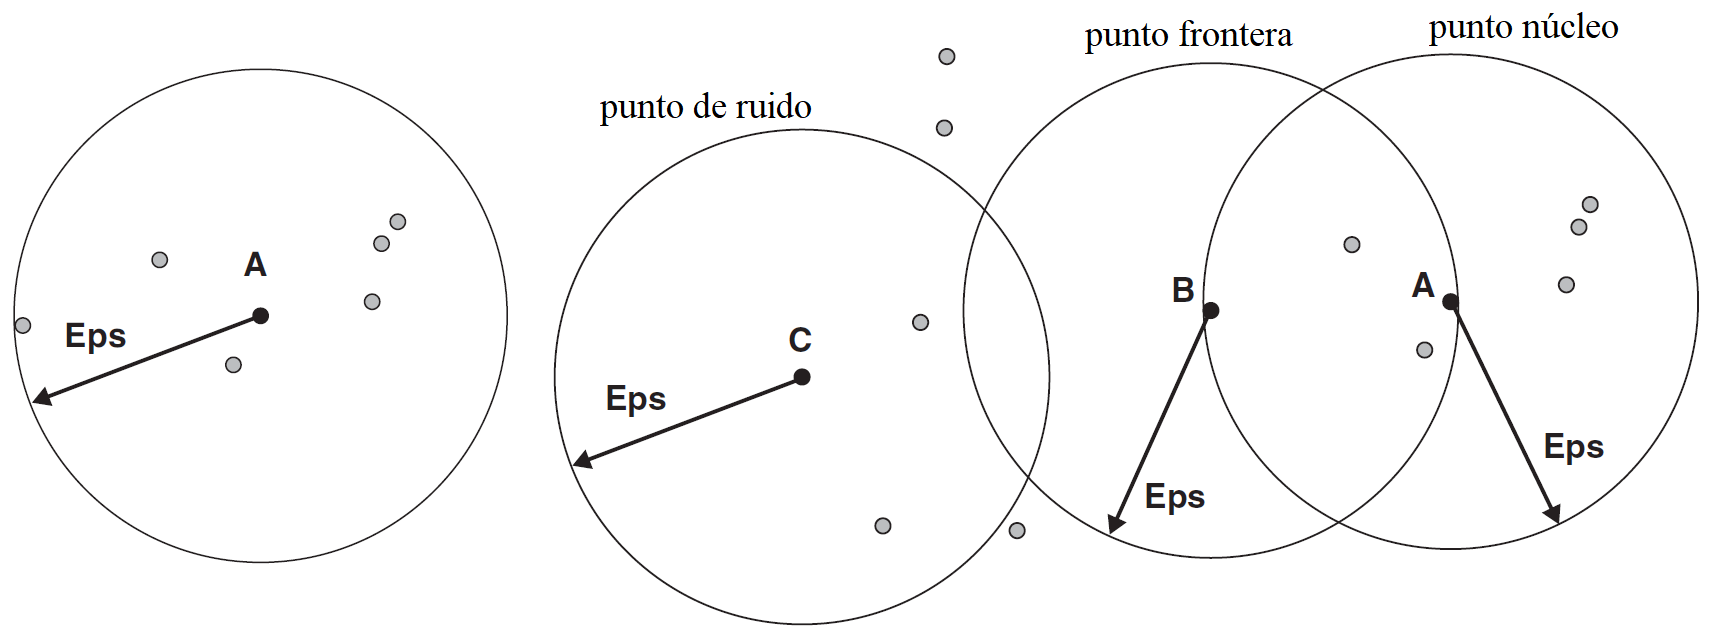
\includegraphics[width=\textwidth]{dbscan.png}
    \caption{Densidad en el entorno de un punto y clasificaciones de los puntos según DBSCAN.}
    \label{img:dbscan}
\end{figure}
